\documentclass[
    paper,
%     manuscript,
%     twocolumn,
%     twoside,
%     revised,
  ]{geophysics}

% Remove once done
\usepackage[textsize=footnotesize, textwidth=2.8cm]{todonotes}

% Additional packages to geophysics.cls
\usepackage[UKenglish]{babel}
\usepackage[utf8]{inputenc}
\usepackage{lmodern}
\usepackage[T1]{fontenc}

\usepackage{amssymb, amsmath, amsfonts}
\usepackage{upquote}
\usepackage[strings]{underscore}
\usepackage{siunitx}                % SI conform commands (eg \num)
\usepackage{tabularx}
\usepackage{colortbl}
\usepackage{booktabs}
\usepackage{xspace}
\usepackage{flafter}

\usepackage[pdftex, final]{hyperref}
% \usepackage[pdftex, hidelinks]{hyperref}
\hypersetup{allcolors=blue, allbordercolors={0 0 .5}, colorlinks=true}

% Figures
\DeclareGraphicsExtensions{.pdf,.png,.jpg}
\renewcommand{\figdir}{./figures}
\ifthenelse{\boolean{@twoc}}{%
  \newcommand{\cwidth}{250pt}}{%
  \newcommand{\cwidth}{240pt}}

\ifthenelse{\boolean{@twoc}}{%
  \newcommand{\acwidth}{250pt}%
  \newcommand{\tcwidth}{250pt}}{%
  \newcommand{\acwidth}{240pt}%
  \newcommand{\tcwidth}{312pt}}

% Own commands
\newcommand{\mr}[1]{\mathrm{#1}}
\newcommand{\emg}[2]{\texttt{emg#1#2}\xspace}
\newcommand{\empymod}{\texttt{empymod}\xspace}
\newcommand{\simpeg}{\texttt{SimPEG}\xspace}
\newcommand{\custem}{\texttt{custEM}\xspace}
\newcommand{\petgem}{\texttt{PETGEM}\xspace}

% Remove once done
\newcommand{\mycom}[2][]{
  \todo[color=yellow]{\textbf{\uppercase{[#1]}}:~#2}}
\newcommand{\imycom}[2][]{
  \todo[inline, color=yellow]{\textbf{\uppercase{[#1]}}:~#2}}
\newcommand{\itodo}[1]{\todo[inline, color=cyan]{\sffamily #1}}
\newcommand{\dul}[1]{\underline{\underline{#1}}}
\newcommand{\ul}[1]{\underline{#1}}
\newcommand{\rmk}[1]{{\color{red}{#1}}}
\newcommand{\ohmm}{\ensuremath{\Omega\,}\text{m}\xspace}

\begin{document}

\title{Open-source landscape for 3D CSEM modelling}

\renewcommand{\thefootnote}{\fnsymbol{footnote}}

\ms{}  % ARTICLE-ID

\address{
\footnotemark[1]TU Delft,
Building 23,
Stevinweg 1 / PO-box 5048,
2628 CN Delft;\\
\footnotemark[2]TODO\\
\footnotemark[3]TODO\\
\footnotemark[4]TODO\\
E-mail: \href{mailto:Dieter@Werthmuller.org}{Dieter@Werthmuller.org};\\
\textbf{Keywords}: CSEM, Open-Source, 3D modelling, FD, FE.
}


\author{%
Dieter Werthmüller\footnotemark[1], %            orcid: 0000-0002-8575-2484
Raphael Rochlitz\footnotemark[2], %              orcid: 0000-0002-5132-916X
Octavio Castillo-Reyes\footnotemark[3], and %    orcid: 0000-0003-4271-5015
Lindsey Heagy\footnotemark[4] %                  orcid: 0000-0002-1551-5926
}

\footer{}
\lefthead{Werthmüller et al.}
\righthead{Open-source 3D CSEM modelling}

\maketitle

%%fakesection ===    ABSTRACT    ===
\begin{abstract}
%
\emph{I will draft a first abstract after the manuscript has been reviewed by
everyone once.}
%
% % Principal objectives and scope of the work
% % Methodology
% % Results
% % Conclusions
%
\end{abstract}

\itodo{
  For comments in the margin, use:\\[.2cm]
  \qquad\texttt{\textbackslash mycom[YOURINITIALS]\{comment\}}\\[.2cm]
  and for inline comments, use:\\[.2cm]
  \qquad\texttt{\textbackslash imycom[YOURINITIALS]\{comment\}}
}

\itodo{
We will have to decide on a Journal. Current suggestions:\\
- GMD: Geoscientific Model Development\\
- SIG: Surveys in Geophysics\\
- SE: Solid Earth\\
- GJI: Geophysical Journal International\\
- GP: Geophysical Prospecting\\
- GEO: Geophysics\\
- CAG: Computers and Geosciences\\
I think \emph{Geoscientific Model Development} and \emph{Surveys in Geophysics}
were the favourite ones when we discussed it ones. I personally would be very
interested in GMD. What do you think? But also interesting would be the GJI,
because the MT comparison was published there, so it would be in the same
place. I just had a very bad experience with GP, so I am not inclined on that
at all.
}

\mycom[RR]{GMD looks very interesting, my only concern is that it might not be in the scope of EM modelers, but we can probably reach modeleres from other communities as well.}

\section{Introduction}

\imycom[RR]{We need to take care to not mix British English with AE, I'm very used to AE, but Dieter started with (at least what I can identify) mainly BE, so I tried to follow (mainly s instead of z and ou instead of o in some words). I hope there are not too many inconsistencies, as probably Lindsey has to fix all these mistakes in the end:-)}

Controlled-source electromagnetic (CSEM) measurements are a frequently applied method in various geophysical exploration fields, such as geothermal and groundwater, oil and gas, mining, civil engineering, or geo-hazards.
Modelling these electromagnetic fields is therefore of great interest to design survey layouts, understand the measured data and inversion purposes.
Publications regarding 3D modelling in electromagnetic methods started to appear as early as the 1970's and 1980's.
These early publications were integral equation (IE) methods, having an anomaly embedded within a layered medium, mostly for loop-loop type transient EM measurements \citep{GJI.74.Raiche, GEO.75.Hohmann, GJI.82.Das, GEO.86.Newman} and magnetotelluric (MT) measurements \citep{GEO.84.Wannamaker}.

In the 1990's, computer became sufficiently powerful that 3D modelling gained traction, which resulted amongst other publications in the book
\emph{Three-Dimensional Electromagnetics} by the SEG
\citep{B.SEG.99.Oristaglio}.
Often cited publications from that time are \cite{RSC.94.Mackie}, 3D MT computation; \cite{RS.94.Druskin}, frequency- and time-domain modelling using a Yee grid and a global Krylov subspace approximation; and \cite{RS.96.Alumbaugh, GJI.97.Newman}, low-to-high frequency computation on massively parallel computers.

The continuous improvement of computing power and the CSEM boom in the early 2000's in the hydrocarbon industry led to a wealth of developed numerical solutions and according publications.
The most common applied methods to solve Maxwell's equation are the IE method \citep{GJI.74.Raiche, RS.02.Hursan, GEO.06.Zhdanov, GP.10.Tehrani,
CAG.16.Kruglyakov, MGS.17.Kruglyakov} and different variations of the
differential equation (DE) method, such as finite differences (FD)
\citep{IEEE.66.Yee, GEO.93.Wang, RSC.94.Mackie, RS.94.Druskin, GEO.09.Streich, CAG.13.Sommer}, finite elements (FE) \citep{GJI.11.Schwarzbach, GEO.04.Commer, GEO.12.daSilva, GJI.13.Puzyrev, GJI.13.Grayver, SEG.16.Zhang}, and finite volumes (FV) \citep{EM.90.Madsen, ECP.07.Haber, GEO.14.Jahandari, PIER.01.Clemens, GP.06.Mulder}.
There are also many different types of discretisation, where the most common ones are regular grids (Cartesian, rectilinear), mostly using a Yee grid \citep{IEEE.66.Yee} or a Lebedev grid \citep{CMMP.64.Lebedev}, but also unstructured tetrahedral grids \citep{SEG.16.Zhang, CAG.17.Cai}, hexagonal meshes \citep{CAG.14.Cai}, or OcTree meshes\citep{ECP.07.Haber}.
Very well written overviews about the different approaches to 3D EM modelling are given by \cite{SG.05.Avdeev} and \cite{SG.10.Borner}.

In the last 15 years, the publications with regards to 3D EM modelling grew tremendously, driven by the ever increasing computing power.
One reason why there are so many reports about this topic results from the variety of solution techniques for the systems of linear equations (SLE).
They can be distinguished between direct solvers \citep{GEO.09.Streich,
GEO.15.Grayver, GP.14.Chung, GEO.14.Jaysaval, SEG.15.Oh, GJI.18.Wang}, indirect solvers \citep{GP.06.Mulder, GJI.15.Jaysaval}, or a combination of both, so-called hybrid solvers \citep{GEO.18.Liu}.
The solvers often use preconditioners such as the multigrid method \citep{SIAM.02.Aruliah, GP.06.Mulder, GJI.16.Jaysaval}.

Probably the main reason for the numerous amount of code developments was already outlined by \cite{SG.05.Avdeev}, who finished his review with the following statement: «\emph{The most important challenge that faces the EM community today is to convince software developers to put their 3-D EM forward and inverse solutions into the public domain, at least after some time. This would have a strong impact on the whole subject and the developers would benefit from feedback regarding the real needs of the end-users.}»
Some major exploration service companies as well as certain research consortia and research groups own their 3D CSEM codes, but how about codes that are open-source?
Academic codes were traditionally often available upon request by authors.
Codes distributed that way were often provided with the request to not share the code, and they often come without a license attached which means that they are not open-source.
Also, at times there can be significant hurdles to install a code.

The meaning of the term open-source evolved rapidly in the last two decades.
Today, open-source generally not only means that a code is available (with a proper license), but also that the code is hosted online, is under version control, has the possibility to file issues and make pull requests to fix bugs. These are important requirements for reproducible research «\emph{to provide the means by which the reader can verify the validity of the results and make use of them in further research}» \citep{GEO.17.Broggini}.
Well maintained codes often have continuous integration that includes testing of the code base and online hosted documentation, often including examples and tutorials.
As such, the term has shifted from purely open-source codes to developments in the open with increasingly building a global community.
Related projects within the realm of geophysical exploration are e.g., pyGIMLi \citep{CAG.17.Rucker} or Fatiando \citep{JOSS.18.Uieda}. \mycom[DW]{Others coming to your mind?}\mycom[RR]{no thoughts about geophysics, but there are many projects for related topics such as gmt, gis, mesh-gen}

\imycom[RR]{i suggest to use also "emph" style for all other package names, not only ours}

We continue addressing the topic of open-source developments with respect to 3D CSEM modeling.
Even though it comprises still the minority of developments, the landscape in this field of research changed in the last five years.
Before, there were only closed-source codes owned by companies or  consortia and individual projects, often without a proper documentation, that could be requested from the authors.
We introduce and compare four recent open-source projects with focus on 3D CSEM modeling.
All presented codes are in the Python ecosystem and use either the FD method on structured grids or the FE method on unstructured tetrahedral meshes.

Furthermore, we deal with the topic of verification.
\cite{GJI.13.Miensopust} presents a review of two workshops dealing with the verification of magnetotelluric forward and inversion codes, but we are not aware of any comparable study or benchmark suite for CSEM data.
Hence, we first conduct a similar exercise for CSEM codes.
We want our efforts to help to ensure the reliability of simulations, not only carried out with the available open-source codes, but also for individual closed-source project.
Analytical and semi-analytical solutions only exist for simple halfspace or layered-Earth models, which served mostly to verify new codes.
Beyond them, the only objective possibility to ensure the accuracy of solutions is by comparing results from different modellers.
If different discretisations and implementations of Maxwell's equations yield the same result, it gives confidence in their accuracy.

We simulate EM fields for a layered background model with vertical transverse isotropy, containing three blocks, and the complex marine Marlim R3D model.
These two model designs as well as the corresponding results from four different codes provide a benchmark for new codes to be compared to and validated with.
In the following section, we introduce the codes under consideration.
Afterwards, we present the considered benchmark cases in detail and present the modeling results of our four codes in terms of accuracy and computational performance.
Beyond that, we extensively discuss important points that control the performance and suitability of our FD and FE codes, including mainly considerations about the mesh design and the choice of solvers. 
We conclude with a summary of our results and a motivation for the EM community to continue not only extending the landscape of open-source codes and also creating a landscape of open-source benchmark models.



\imycom[RR]{Regarding "It is worth mentioning that there are many more 3D EM codes developed in other fields than geophysics such as communication systems (antennas, radar, satellites), medical imaging, or civil engineering.
	There are various open-source codes in these fields too, e.g., Elmer ([DW]: Add 2-3 proper references) (\href{http://www.csc.fi/elmer}{csc.fi/elmer}, couldn't find a publication, just a poster).
	While these codes could potentially be used for the same goals as presented here we restrict our review to codes purpose-built and ready without further adjustments for geophysical applications."
	
	I thought a lot about this but I just think the previous paragraph is not required in our introduction and haven't find a location where it fits considering different logical structures. I think it is also not important for this paper to tell "that there are more codes in EM than only geophysics", that's quite obvious. Maybe delete or shorten to 1 sentences to add Elmer and place this sentence somewhere else? I think, an appropriate list of all non-geophysical open-source EM codes should be very long anyway, we just don't know them or at least I'm not familiar with them.}



\clearpage  % TODO: Just for now while drafting, remove later!
\section{Codes}

\imycom[RR]{I think we should introduce the term degrees of freedom (dof), equivalent to the size of the SLE, as general measure of our problem sizes. If it is somewhat x*Nedges, or related to Ncells or Nnodes, who cares? We just need this one number for this paper in my opinion, more details in the jupyter notebooks - fine.}

The four codes under consideration are, in alphabetical order, \custem \citep{GEO.19.Rochlitz}, \emg3d \citep{JOSS.19.Werthmuller}, \petgem \citep{GJI.19.CastilloReyes}, and \simpeg \citep{CAG.15.Cockett}.
All four codes have their user-facing routines written in Python; all of them make heavy use of \texttt{NumPy} \citep{CSE.11.VanDerWalt} and \texttt{SciPy} \citep{NM.20.Virtanen}.
The four of them are “modern” open-source projects, meaning that they come with both, an open-source license and an online-hosted version-control system with tracking possibilities (raising issues, filing pull requests).
All developments comprise an extensive online documentation with many examples and have continuous integration to some degree.
Newer package-management systems such as Conda, Docker, or pip significantly supported us to make our codes easily available and installable without any user-side compilations.
Each one can be downloaded and installed with a single command.

In the following a quick rundown of the codes.
It is, however, beyond the scope of this article to go into every detail of the different modellers, and we refer to their documentations for more details.
An overview comparison of the different codes is given in Table~\ref{tbl:codecomparison}.
All codes have in common that they solve the\mycom[DW]{are we all using the weak form?} weak formulation of Maxwell's equation in its differential form (DE) under the quasistatic or\mycom[DW]{are we all using the diff. approx?} diffusive approximation, hence neglecting displacement currents.
The machines on which the different codes were run are listed in Table~\ref{tbl:machines}, together with the responsible operator.

\imycom[RR]{too much info (redundancy to text) for table caption}

\tabl[btp]{codecomparison}{All codes solve the weak form of Maxwell's equations in its differential form (DE) under the quasistatic approximation. Note that \emg3d is a solver on its own, while the other codes implement third-package solvers such as \texttt{PETSc} \citep{Preprint.Abhyankar}, \texttt{MUMPS} \citep{SIAM.01.Amestoy}, or \texttt{PARDISO} \citep{FGCS.04.Schenk}.
}{
  \centering
  \footnotesize
\begin{tabularx}{\linewidth}{lXXXX}
  \toprule
  %
  & \custem & \emg3d & \petgem & \simpeg  \\
  \midrule
  %
  Home & \href{https://custem.rtfd.io}{custem.rtfd.io}
       & \href{https://empymod.github.io}{empymod.github.io}
       & \href{http://petgem.bsc.es}{petgem.bsc.es}
       & \href{https://docs.simpeg.xyz}{simpeg.xyz} \\
  License & GPL-3.0 & Apache-2.0 & GPL-3.0 & MIT \\
  Installation & \texttt{conda}
               & \texttt{pip}; \texttt{conda}
               & \texttt{conda}
               & \texttt{pip}; \texttt{conda} \\
  Comp. Dom. & frequency \& time & frequency & frequency & frequency \& time \\
  Method & FE & FV & FE & FV \\
  Mesh & tetrahedral & rectilinear & tetrahedral & recti- \& curvilinear \\
  BC & PMC; PEC & PEC & PEC & PEC; PMC \\
  Solver & \texttt{MUMPS} & \emg3d & \texttt{PETSc}; \texttt{MUMPS} &
           \texttt{PARDISO}; \texttt{MUMPS} \\
  %
  \bottomrule
\end{tabularx}}%
%

%
\tabl[btp]{machines}{List of computer and operating system (hardware and
software) on which the different codes were run, together with the operator.}{
  \centering
  \footnotesize
  \begin{tabularx}{\linewidth}{lXl}
  \toprule
  %
  Code & Computer and Operating System & Operator \\
  \midrule
  %
  \custem & PowerEdge R940 server; 144 Xeon Gold 6154 CPU @2.666 GHz; ~3 TB
            DDR4 RAM; Ubuntu 18.04
          & Raphael Rochlitz \\
  \emg3d  & Laptop; i7-6600U CPU@2.6 GHz x4; 16 GB of memory, Ubuntu 18.04
          & Dieter Werthmüller \\
  \petgem & Marenostrum4. Intel Xeon Platinum from Skylake generation; 2
            sockets Intel Xeon Platinum 8160 CPU with 24 cores each @2.10GHz
            for a total of 48 cores per node; 386 Gb DDR4 RAM per node; SuSE
            Linux Enterprise
          & Octavio Castillo-Reyes \\
  \simpeg & ???
          & Lindsey Heagy \\
  %
  \bottomrule
\end{tabularx}}%
%


\itodo{
Each code should be briefly summarized by three points:\\
- Brief intro\\
- Main selling point\\
- Planned features\\
I think in a first round \textbf{everyone should just write what they want to
write and think is important for their code}. In a second round we should then
homogenize it, such that all codes have more or less the same length/weight and
also similar topic/layout.
}

\clearpage  % TODO: Just for now while drafting, remove later!
\subsection{custEM}

The customisable electromagnetic modeling Python toolbox custEM was developed for simulating arbitrary complex 3D CSEM geometries with focus on semi-airborne setups, but it supports also land-based, airborne, coastal  or marine environments.
Multiple electric or magnetic field or potential finite-element approaches were implemented as total or secondary field formulations.
The finite-element kernel, including higher order basis functions and parallelisation, relies on the FEniCS project \citep{B.SPR.12.Logg, B.SPR.16.Langtangen}.
The resulting systems of linear equations are solved with MUMPS \citep{SIAM.01.Amestoy}, which is a very robust but memory consuming choice. 
Primary field solutions are supplied by the COMET \citep{GEO.20.Skibbe} package.

The toolbox considers generally anisotropic petrophysical properties.
Even though changes of the conductivity is mainly of interest for CSEM modeling, the electric permittivity and magnetic permeability can be taken into account using the preferred electric field approach on Nédélec elements.
Recently, induced polarization parameters in frequency-domain and three methods for simulating time-domain responses were added to custEM.
The provided meshing tools based on TetGen \citep{TOM.15.Si} and functionalities of pyGIMLi \citep{CAG.17.Rucker} facilitate the generation of tetrahedral meshes including layered-earth geometries with topography or bathymetry and anomalous bodies which are allowed to be connected or to reach the surface.

The custEM toolbox is under steady development and maintenance.
Future enhancements comprise adding iterative solution techniques, provided by FEniCS, as well as further functionalities for automatically incorporating intersecting bodies such as folds or faults in meshes. 
Furthermore, current work is on using custEM for inverse modeling applications. 



\subsection{emg3d}

The 3D CSEM modeller \emg3d is a multigrid \citep{CMMP.64.Fedorenko} solver for
3D electromagnetic diffusion following \cite{GP.06.Mulder}, with tri-axial
electrical anisotropy, isotropic electric permittivity, and isotropic magnetic
permeability. The matrix-free solver can be used as main solver or as
preconditioner for one of the Krylov subspace methods implemented in SciPy, and
the governing equations are discretized on a staggered grid by the
finite-integration technique \citep{AEU.77.Weiland}, which is a finite-volume
generalization of a Yee grid. The code is written completely in Python using
the NumPy and SciPy stacks, where the most time- and memory-consuming parts are
sped up through jitted (just-in-time compiled) functions using Numba
\citep{LLVM.15.Lam}. The code computes the electric field due to an electric
source in the frequency-domain, which is its main application (frequency-domain
CSEM). However, there are also routines to obtain the magnetic field due to an
electric source, to obtain the electric and magnetic fields due to a magnetic
source, and to obtain time-domain responses.

The multigrid method is characterized by almost linear scaling both in terms of
runtime (CPU) and memory (RAM) usage, and it is therefore a comparably
low-memory consumption solver. It is also minimal in terms of requirements,
only NumPy, SciPy, and Numba are required, with Python 3.7+. The current
development is focused on adding basic inversion capabilities, and a further
plan is to implement a hook in order to use \emg3d as a frequency-domain CSEM
solver within the grander \simpeg framework.

\subsection{PETGEM}

TODO


\subsection{SimPEG}

TODO


\clearpage  % TODO: Just for now while drafting, remove later!
\section{Numerical Verifications}

We computed the responses for two different models to verify that all different 3D codes yield the same electromagnetic responses.
The first simple Block model consists of a layered, anisotropic
background with three embedded blocks.
The second Marlim R3D model is based on a very complex, realistic marine CSEM setup.

\subsection{Block model}

\imycom[RR]{I think the miensopust argument is rather suited to motivate our work in the introduction, i hope its fine that i moved this argument}

The block model is a derivation of the \emph{Dublin Test Model 1} from the first EM modeling workshop described by \cite{GJI.13.Miensopust}.
We took the same layout of the blocks but adjusted the dimensions and resistivities to a typical marine CSEM problem, as shown in Figure~\ref{fig:block-model}.
We additionally added a layered background with vertical transverse isotropy (VTI).
%
\plot*{block-model}{width=.6\textwidth}{
  Sketch of the block model. The layered model consists of an air layer, a
  water layer, a thin top-layer followed by a thick, anisotropic background
  layer, and at the bottom a resistive basement layer. All three blocks are
  embedded in the thick background layer, which has VTI with
  $\lambda=\sqrt{2}$.
}
%

The layered model consists of an upper halfspace of air, a 600\,m deep water
layer, followed by a 150\,m thick, isotropic layer of 1\,\ohmm, a 3.3\,km
thick, anisotropic layer of $\rho_\text{h}=2\,\ohmm$ and
$\rho_\text{v}=4\,\ohmm$, and finally a resistive basement consisting of a
lower halfspace of $1000\,\ohmm$. The 200\,m long, $x$-directed source is
located 50\,m above the seafloor from $x=-50$ to $x=50\,$m in $x$-direction, at
$y=0\,$m. The $x$-directed receivers are placed on the seafloor every 200\,m
from $x=-10\,$km to $x=+10\,$km in three lines for $y=-3, 0, 3\,$km.

The thin isotropic layer beneath the water requires many tetrahedra for a good-quality discretisation. Therefore, the FE codes custEM and PETGEM used the same tetrahedral mesh with a horizontal layered-earth extent of 30\,km from the origin, surrounded by a ten times larger halfspace-like boundary mesh with water conductivities assigned to the subsurface.
This approximation significantly reduced the problem size compared to considering the layered-earth geometry for the whole computational domain.
\imycom[RR]{Add short information about mesh design with SIMPEG and emg3d, including something like "comparatively coarse discretization in center to minimize computation times" }

In a first step, we compare the layered background to the semi-analytical solutions of a 1D code, for which we use  \empymod\citep{GEO.17.Werthmuller}.
Figures~\ref{fig:results-layered-0} and \ref{fig:results-layered--3} show the actual responses in the top rows, and the relative error in the bottom rows for the receiver lines $y=0\,$km and $y=\pm3\,$km, which are identical.

Figure~\ref{fig:results-layered-0} illustrates the inline responses in the top-row for offsets $r>0.5\,$km. We only show the
semi-analytical result for the real and imaginary amplitudes.
The bottom row displays the relative error of the 3D codes.
The results show that all codes are yielding accurate result with errors of around 1\,\% in most parts and overall below a few percent, disregarding locations affected by sign reversals.
The differences can be mainly attributed to the chosen discretisations.
The FE codes show the strongest misfits at large offsets, most likely caused by the utilized boundary mesh, whereas \emg3d seems to do a very good job\mycom[RR]{maybe reformulate to something like: whereas emg3d appears to be not affected by boundary effects}.
Close to the 200\,m long source, emg3d is less precise which is attributed to comparatively large cell sizes in this region.
%
\plot*{results-layered-0}{width=.8\textwidth}{
   Comparison of the layered model for the inline receivers ($y=0\,$km).
   Top row shows the semi-analytical responses from \empymod, and bottom row
   shows the relative error (\%) of \custem, \emg3d, \petgem, and \simpeg.
}
%

\imycom[RR]{I suggest to show y-component for broadside and the errors of the weak component (if not too bad), otherwise only broadside is required to save a plot, because inline should be better for Ex in general.}
The corresponding broadside responses for $y=\pm3\,$km are shown in Figure~\ref{fig:results-layered--3}.
The CPU and RAM requirements are listed in Table~\ref{tbl:comp-layered}.
%
\plot*{results-layered--3}{width=.8\textwidth}{
   Comparison of the layered model for the broadside receivers ($y=-3\,$km).
   Top row shows the semi-analytical responses from \empymod, and bottom row
   show the relative error (\%) of \custem, \emg3d, \petgem, and \simpeg.
}
%

%
\tabl[btp]{comp-layered}{Comparison of used CPU and RAM and of number of cells
  used to discretize the layered model. \imycom[DW]{I will fill this table out
  once we all submitted the final versions of the results.}}{
  \centering
\begin{tabular}{c c c c c}  %{lS[table-format=4.2]rS[table-format=4.2]rl}
  \toprule
  %
  Code & {CPU} & \#Procs & RAM     & \#dof \\
       & {(s)} &         & {(GiB)} &         \\
  \midrule
  %
  \custem & 0.0 &  0 & 0.0 & 0 \\
  \emg3d  & 0.0 &  0 & 0.0 & 0 \\
  \petgem & 0.0 &  0 & 0.0 & 0 \\
  \simpeg & 0.0 &  0 & 0.0 & 0 \\
  %
  \bottomrule
\end{tabular}}%
%


In a second step, three resistive blocks were added in the 3.3\,km-thick, anisotropic background layer as shown in Figure~\ref{fig:block-model}.
They have resistivities of $\rho=10\,\ohmm$ (shallow beam perpendicular to survey lines), $\rho=100\,\ohmm$ (thin plate, South-East), and $\rho=500\,\ohmm$ (cube, North-West).
As there are no analytical solutions for this model we show the normalized difference between different codes, instead of the relative error, where the normalized difference of two responses $p$ and $q$ is given by
%
\begin{equation}
  \mr{NRMSD~(\%)} = 200 \frac{|p - q|}{|p| + |q|}\ .
  \label{eq:nrmsd}
\end{equation}
%
\imycom[DW]{NRMSD: Comparing all codes to all would make the figures too cluttered, and I don't think it would add a lot insights. My idea is therefore to compare \emg3d/\simpeg (the two FV ones), \custem/\petgem (the two FE ones), and \emg3d/\custem (a cross-comparison). What do you think?}

\imycom[RR]{Agreed. Another suggestion, I solved this visualization problem with a color coded matrix plot, showing 90th percentiles or median values of all errors along the line as meaningful comprehensive number. Look in my thesis - example 4. Comparison for real and imag could be in the lower and upper triangles, or we show absolute magnitudes for layered earth in lower triangle and for block model in upper triangle. With help of this plot, one could easily say if differences are higher for block model and which codes fit to each other well.}

\imycom[RR]{If using the mentioned matrix plots, we would need only one of the figures 4-6, and could show the other data comprehensively.
I added a python script to generate an example of my plotting suggestion in the model-block directory and a new Figure 7 in the manuscript that illustrates what I mean. Of course, any upgrade suggestion for this initial idea is welcome, aside from making it looking nice with labels  and annotations.}

The results for the three receiver lines $y=-3,0,3\,$km are shown in Figures~\ref{fig:results-block--3}, \ref{fig:results-block-0}, and \ref{fig:results-block-3}, respectively, and the corresponding CPU and RAM in Table~\ref{tbl:comp-block}.
We can conclude from the NRMSD that similar codes have a smaller NRMSD than cross-comparison, hence \emg3d and \simpeg are very similar, as well as are \custem and \petgem.
\mycom[DW]{Write in detail when all results are available}
%
\plot*{results-block--3}{width=.8\textwidth}{
   Comparison of the block model for the broadside receivers at $y=-3\,$km.
   Top row shows the responses and bottom row the NRMSDs (\%)
   between \emg3d--\custem, \custem--\petgem, and \emg3d--\simpeg.
}
%

%
\plot*{results-block-0}{width=.8\textwidth}{
   Comparison of the block model for the inline receivers at $y=0\,$km.
   Top row shows the responses and bottom row the NRMSDs (\%)
   between \emg3d--\custem, \custem--\petgem, and \emg3d--\simpeg.
}
%

%
\plot*{results-block-3}{width=.8\textwidth}{
   Comparison of the block model for the broadside receivers at $y=+3\,$km.
   Top row shows the responses and bottom row the NRMSDs (\%) between
   \emg3d--\custem, \custem--\petgem, and \emg3d--\simpeg.
}
%

%
\tabl[btp]{comp-block}{Comparison of used CPU and RAM and of number of cells
  used to discretize the block model. \imycom[DW]{I will fill this table out
  once we all submitted the final versions of the results.}}{
  \centering
\begin{tabular}{c c c c c}  %lS[table-format=4.2]rS[table-format=4.2]rl}
  \toprule
  %
  Code & {CPU} & \#Procs & RAM     & \#dof \\
       & {(s)} &         & {(GiB)} &         \\
  \midrule
  %
  \custem & 0.0 & 24 & 0.0 & 0 \\
  \emg3d  & 0.0 &  1 & 0.0 & 0 \\
  \petgem & 0.0 & 48 & 0.0 & 0 \\
  \simpeg & 0.0 &    & 0.0 & 0 \\
  %
  \bottomrule
\end{tabular}}%
%

The difference becomes only significant at offsets larger than 8\,km. This is due to a practical difference in the meshing: This simple block model
is advantageous for FV codes, as it consists of rectangular blocks and
horizontal layers, simple geometric objects. While having a very thin, shallow
layer is straight-forward for FV codes, it requires many cells for a FE code.
The thin layer was therefore limited in its horizontal extent
to\mycom[DW]{Raphael, to what x/y exactly?} ???. This is the reason for the
increased NRMSD at large offsets, and it has nothing to do with the accuracy of
the computation itself.\mycom[RR]{see imycom below figure 6}

\imycom[RR]{60 x 60 km (30 km in each direction from center). I already added a paragraph about mesh generation in the beginning, I suggest to remove this description here and jsut refer to like "Similar to the layered earth model, the largest errors occur at offsets $>8$\,km due to the differences in mesh design."
We should also mention that relative errors are related to the magnitudes, as real is so much weaker at larger offsets, it is clear that errors increase significantly. Alternatively, we could show absolute magnitude or phase errors such as in the Marlim model.}


\begin{figure}
	\centering
	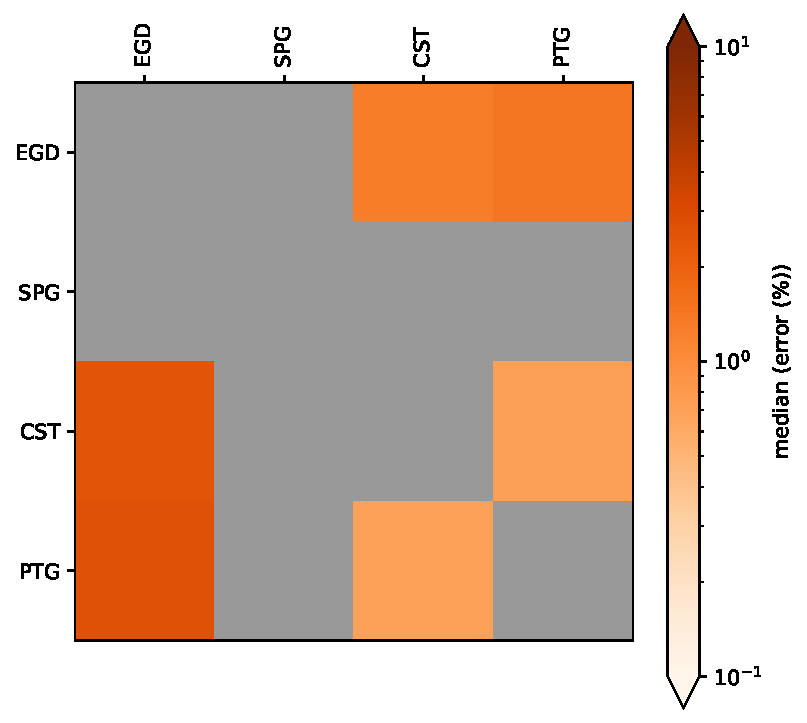
\includegraphics[width=5cm]{figures/median-stats-block--3.pdf}\hfill
	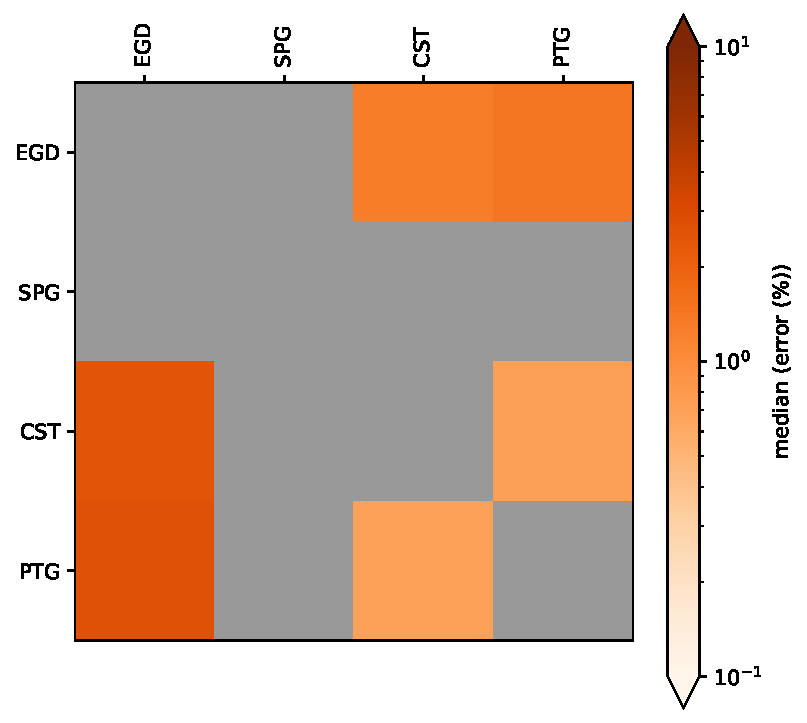
\includegraphics[width=5cm]{figures/median-stats-block-0.pdf}\hfill
	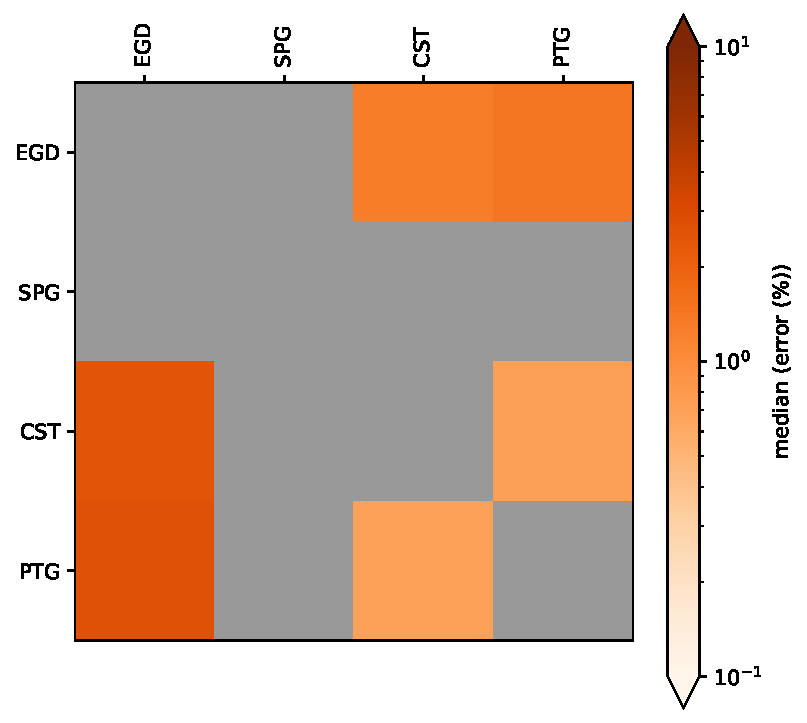
\includegraphics[width=5cm]{figures/median-stats-block-3.pdf}
	\caption[Median errors]{Overall misfit relations between all codes for the three receiver lines y=-3, y=0 \& y=3 f.l.t.r. Colors indicate the median values of the 101 calculated NRMSD arguments for each line between all codes. Errors for real parts are shown in the lower triangle, for imaginary parts in the upper triangle.}
	\label{medianmisfits}	
\end{figure}



\clearpage  % TODO: Just for now while drafting, remove later!
\subsection{Marlim R3D}

The Marlim oil field is a giant reservoir in a turbidite sandstone horizon in the north-eastern part of the Campos Basin, offshore Brazil, which was discovered in 1985.
\cite{BJG.17.Carvalho} created from seismic data and well log data a realistic resistivity model with vertical transverse isotropy (VTI), Marlim R3D (MR3D), which they released under an open-source license. 
\cite{GEO.19.Correa} computed CSEM data for six frequencies from 0.125\,Hz to 1.25\,Hz, released under an open-source license.
To compute the data they used a state-of-the-art code from the industry \citep{GEO.07.Maao}.
It is therefore an ideal case to verify our open-source codes against, as it is a complex, realistic model and the data were computed by an industry-proofed code.\mycom[RR]{I would delete this sentence, not that important and a bit redundant}
Additionally, that code is a time-domain code, whereas the four codes under consideration here compute the results all in the frequency-domain.

The detailed reservoir model consists of 1022 by 371 by 1229 cells, totalling to almost 466 million cells, where each cell has dimensions of 25 by 75 by 5\,m.
For the computation the model is upscaled to 515 by 563 by 310 cells, totalling to almost 90 million cells, where each cell has dimensions of 100 by 100 by 20\,m.

The published data set consists of a regular grid of receivers of 20 in eastern direction by 25 in northern direction, 500 receivers in total, with 1\,km spacing located on the irregular seafloor.
45 source-towlines were located on the same grid, 50\,m above the seafloor, with shots every 100\,m. In
\cite{GEO.19.Correa} the actual responses for one receiver with the corresponding East-West inline and one East-West broadside acquisition line are shown, which is the data we chose for our comparison.
The cross-section of the resistivity model along the chosen inline acquisition line is shown in Figure~\ref{fig:model-marlim}, together with the acquisition information.

\imycom[RR]{I used gmt the last time 7 years ago , in between I tried the gmt4py tools, but they did not work well on my machine. I suggest to use two plots next to each other, a similar figure as in the notebook and a simple x-y coord sketch (identical extent as the bird perspective view in the other plot) with all Tx / Rx locations, highlighting the relevant line and Rx for us.}

%
\plot*{model-marlim}{width=\textwidth}{
  This figure obviously needs to be improved massively (at least a colorbar).
  What would you like to show from the actual data here?
  A nice figure would  be Figure 2 in \cite{GEO.19.Correa}; however, note that
  the drawn survey line in that figure are plainly wrong. If someone is
  familiar with GMT and happy to make that would be great. Also, the
  cross-section is currently heavily vertically exaggerated.
}
%

We computed all all six frequencies for all components ($E_x$, $E_y$, $E_z$)
for both inline and broadside acquisition lines. However, we show here only
the three frequencies and the responses with the strongest amplitudes (which
are generally used in processing), which are $E_x$ inline and broadside and
$E_y$ broadside. The comparison is shown in Figure~\ref{fig:results-marlim}.
%
\plot*{results-marlim}{width=\textwidth}{
  This is one heck of a figure. Just an idea, please make suggestions how to
  improve it (currently, \petgem data is a copy of \custem data, and \simpeg
  data is a copy of \emg3d data).
}
%


\imycom[DW]{There are some interesting features we should highlight. But again,
we first need all results. E.g.}
\begin{itemize}
  \item 0.125\,Hz: on the left side, \custem and \emg3d are almost identical,
    but very different from MR3D. So there I actually trust more our
    calculation, or there is a difference in the model that we did not take
    into account.
  \item 0.125\,Hz: on the right side, \custem is very similar to MR3D, whereas
    \emg3d is off.
  \item 0.125\,Hz and 0.5\,Hz: on the right side, \custem seems to very similar
    to MR3D.
\end{itemize}



%
\tabl[btp]{comp-marlim}{Comparison of used CPU and RAM and of number of cells
  used to discretize the Marlim R3D model. \imycom[DW]{I will fill this table
  out once we all submitted the final versions of the results.}}{
  \centering
\begin{tabular}{c c c c c}  %{ls[table-format=4.2]rs[table-format=4.2]rl}
  \toprule
  %
  Code & {CPU} & \#Procs & RAM     & \#dof \\
       & {(s)} &         & {(GiB)} &         \\
  \midrule
  %
  \custem & 0.0 &  0 & 0.0 & 0 \\
  \emg3d  & 0.0 &  0 & 0.0 & 0 \\
  \petgem & 0.0 &  0 & 0.0 & 0 \\
  \simpeg & 0.0 &  0 & 0.0 & 0 \\
  %
  \bottomrule
\end{tabular}}%
%


\clearpage  % TODO: Just for now while drafting, remove later!
\section{Discussion}
%
% enago.com/academy/discussion-conclusion-know-difference-drafting-manuscript/
%
% In order to make your discussion section engaging, you should include the
% following information:
% - The major findings of your study
% - The meaning of those findings
% - How these findings relate to what others have done
% - Limitations of your findings
% - An explanation for any surprising, unexpected, or inconclusive results
% - Suggestions for further research
%
% Your discussion should NOT include any of the following information:
% - New results or data not presented previously in the paper
% - Unwarranted speculation
% - Tangential issues
% - Conclusions not supported by your data
%

\imycom[DW]{Maybe we should create a Google-Doc for working on the Discussion
collaboratively at the same time?}

\imycom[RR]{if you prefer ok, but I don't think this is necessary, if everyone adds the own thoughts when he receives the manuscript. Same for conclusions. We need to take care to not mix discussion and conclusions, some of the statements from here belong rather to the conclusions, I hope it's fine that I reorganized the content. Aside from that, I already added all thoughts of mine.}

Even if modeling results may look completely valid, they could not be correct at all.
Verifying the performance of 3D CSEM codes for real 3D problems is only possible by cross-validating multiple solutions.
Overall, we observed an excellent match between all solutions.
The relative misfits, almost always smaller than 10\,\%, were related to the either weak or strong amplitudes of real or imaginary parts and can be attributed to particularities regarding the discretization, boundary effects, and interpolation.
Considering this satisfactory result in terms of accuracy and robustness, it is more interesting to discuss the characteristics of the four considered codes with focus on the demand of computational resources and the capability of handling the investigated CSEM geometries, including the very important underlying mesh design.
The following arguments are based on a comparison of only marine CSEM models, which are the focus of industry applications.
Nevertheless, we are confident that many observations would hold in a similar manner for land-based, airborne, or mixed setups. 

We point out that making a synthetic and a real benchmark model available to cross-validate any 3D CSEM code was the determining reason for their choice, regardless of the suitability of the considered FD and FE codes for these problems.
The first model, including the block-anomalies variation, is exactly reproducible by using any numerical method with either regular or irregular computational domains.
Aside from the idea of analyzing an industrially relevant benchmark example, the Marlim R3D model was also considered since the primary design from \cite{GEO.19.Correa} uses a regular discretisation. 
At least theoretically, the exact geometry might be reconstructed with unstructured meshes, but it is never possible to convert an irregular geometry to a regular grid without approximations.
Hence, the chosen examples favoured the finite-difference codes, since they used either regular grids or octree-meshes, whereas the two finite-element codes were required to tetrahedralise the model geometries.

In the first model, the necessity of discretising regular structures with tetrahedra, especially thin layers, led to comparatively large FE problem sizes and computational resource demands.
FE codes with unstructured meshes were probably the poorest choice of all commonly used methods for this setup in terms of computational performance.
However, thinking about introducing just one slight irregularity such as bathymetry, a thin dipping plate or an anticline, the performance behaviour could likely switch.
All of these changes would barely change the problem size for the FE codes, but significantly increase it for the FD codes if the true geometry should be approximated sufficiently accurate.

The real Marlim R3D model was, ironically, the ideal case for FE codes because it's structure was characterized by irregular lithological horizons obtained from seismic data.
Since the corresponding published resistivity model was defined on a regular grid, we were forced to approximate the comparatively fine regular discretization by an unstructured one and interpolate the resistivity data for being able to apply the FE codes to this problem.
We are completely aware about the ineptness of this re-approximation procedure, unless it served for the cross-validation purposes.
Nevertheless, the chosen tetrahedral discretization, especially in combination with second order basis functions, showed clearly the intrinsic strength of the FE codes, requiring significantly less dof for meshing irregular geometries in general. The p2 FE solution required only $\approx$9\,M dof instead of $\approx$90\,M dof for the FD system by \citet{GEO.19.Correa}, disregarding the structure of the system matrices.

The codes under consideration use direct and indirect solvers. In general, the biggest advantage of iterative solvers with appropriate preconditioners are the comparatively small memory requirements.
Direct solvers can be considered as most robust to solve any ill-conditioned SLE, which is most important for systems of the FE method on unstructured meshes.
As the consumed computational resources indicate, a more powerful machine than a laptop is required for most 3D CSEM problems, but no high-performance-computing architecture.

The computation times can differ significantly for specific simulations, but there is no clear general advantage for one of the solver types. 
In our models, the runtime comparison favoured the iterative solver and therefore, \emg3d.
Even though not shown here, direct solvers exhibit their strongest advantage in terms of computation times if responses of multiple CSEM transmitters need to be calculated in the same computational domain.
As the system matrix factorisation requires 98-99\,\% of the solution time, computations for additional sources come at almost no cost for direct solvers, i.e., MUMPS, whereas it would come at the same cost as the first source for \emg3d.
For the sake of completeness, note that there are also advanced techniques for iterative solvers to make use of preconditioners, factorisations, or intermediate solutions of the previous SLE to speed up the calculation for multiple sources, but this argumentation is beyond the scope of this work.

We see this work as the start for future elaboration on the validation of modeling codes, not necessarily restricted to CSEM problems.
Much more comparisons and examples are required which not only result in the finding that a sufficient accuracy was observed. 
3D CSEM modelling is a difficult task, which requires many considerations. It starts with the selection of the right code for the problem. 
We found that the meshing task, which is most performance determining, is particularly difficult and relevant, choosing cells small enough to appropriately represent the model yet to be as coarse as possible still achieving the desired precision.
The required model extent has to be considered as well, thinking also about effects of the so-called airwave in marine setups or boundary meshes in general.
This is not a new finding but rather well known fact.
We are surprised that only the minority of publications in the field of 3D EM modeling considers a sufficiently detailed elaboration of the meshing process.

A completely objective evaluation of codes is only possible by cross-validation.
Nevertheless, we point out that using different discretizations or formulations of the numerical approach, e.g. by choosing field or potential approaches, second or total field formulations, different polynomial order basis functions, and others, is a suitable alternative to the cross-comparison of multiple codes for self-validating complex 3D results.
This is a very powerful method to confirm the general functionality of codes for any modeling problem, which might not be covered by existing cross-validation benchmark examples.
Considering for instance  this study, it would be very optimistic to estimate the accuracy of the utilized codes for a land-based mineral exploration setup with a highly-conductive, steeply-dipping conductor.  
However, each modeller could run multiple simulations with different configurations to increase the reliability of the obtained results.

\imycom[DW]{I would like to capture as many as possible of the (I) differences,
	(II) difficulties, (III) advantages, and (IV) disadvantages, that we
	encountered in this exercise. This includes differences from direct to
	iterative solver and differences from FE to FD codes etc. Please just jot down
	things that come to your mind.}

\clearpage  % TODO: Just for now while drafting, remove later!
\section{Conclusions \& Outlook}
%
% enago.com/academy/discussion-conclusion-know-difference-drafting-manuscript/
%
% Your conclusion should:
% - Restate your hypothesis or research question
% - Restate your major findings
% - Tell the reader what contribution your study has made to the existing
%   literature
% - Highlight any limitations of your study
% - State future directions for research/recommendations
%
% Your conclusion should NOT:
% - Introduce new arguments
% - Introduce new data
% - Fail to include your research question
% - Fail to state your major results
%

\imycom[DW]{Maybe we should create a Google-Doc for working on the Conclusions
collaboratively at the same time?}

\imycom[DW]{I obviously haven't really done this section, just af few thoughts
that I noted over time. I think the discussion (as the abstract) has to be
tackled once the rest is at least in a draft status and all data is ready.}

\imycom[RR]{I also rearranged some of your thoughts and formulated mine. I moved some of them (the few sentences that were rather redundant motivation content) to the introdcution.}

We compared four different open-source 3D CSEM modellers by computing responses for a layered, anisotropic model, including a modification with three resistive blocks, and the realistic marine Marlim R3D model.
All comparisons exhibited an excellent reliability of the solutions.
Our data should make it very easy for new codes to have a readily available data set to test against and verify.
We are confident that the discussions about runtimes, memory consumptions, solver choices, and, most important, discretisations of the 3D CSEM problems help potential users not only to decide which modeller is best suited for specific tasks, but also to support their individual projects.

As none of the considered methods is best suited for all problems,
it is important to have more test models for various scenarios in future.
Our study is limited to marine CSEM cases in the frequency-domain.
Reasonable extensions include providing benchmark models for land, airborne, or mixed CSEM environments as well as time-domain data.
Another addition to this work would be focusing on complex irregular  models, tailored for an FE or FV code based on unstructured meshes, and to compare how the FD codes can cope with it.

We encourage the community to not only work on new open-source code developments but also to create a landscape of easily accessible benchmark models for increasing the number of reliable and reproducible solutions.
Our study could provide one of the primary inputs for this task.  
We are confident that the mentioned development will and should be taking place, taking into account the current general trend in science to open-source papers, codes or data.




\clearpage  % TODO: Just for now while drafting, remove later!
\section{Acknowledgment}

\imycom[DW]{Write here your fundings; and potentially also minor contributors
etc.}

We would like to thank Paulo Menezes for the help and explanations with regards to the Marlim R3D model and corresponding CSEM data, and for making their actual computation model available under an open-source license.

The work of D.W. was conducted within the Gitaro.JIM project funded through MarTERA, a EU Horizon 2020 research and innovation programme (No 728053); \href{https://www.martera.eu}{martera.eu}.
The development of custEM as part of the DESMEX project was funded by the Germany Ministry for Education and Research (BMBF) in the framework of the research and development program Fona-r4 under grant 033R130D.

\clearpage  % TODO: Just for now while drafting, remove later!
\section{Data}

All files to rerun the different models with the four codes and reproduce the shown results are available at \dots.
\itodo{Put up on Zenodo, link here.}


\clearpage  % TODO: Just for now while drafting, remove later!
% REFERENCES
\bibliographystyle{Refs}          % Modified SEG bibliography style.
\bibliography{Refs}

\end{document}
